\section{Word Embeddings} \label{sec:WordEmbeddings}


\subsection{Usage of Word Embeddings in Natural Language Processing} \label{sec:WordEmb_Useage}


\textbf{Word embeddings} are fixed-length vector representations of words that have led to the success of many NLP systems in recent years, across tasks like \nameref{nlptask:namedentityrecognitionNER}, \nameref{nlptask:semanticparsingSP}, \nameref{nlptask:postagging}, and \nameref{nlptask:semanticrolelabelingSRL} (Luong et al. 2013, p. 1).

A key idea in NLP is suggests that information lives in text corpora and people and machines can use programs to collect and organize this information for use in NLP. 

A second key idea in linguistics is that words used in similar ways have similar meanings (Firth, 1957). Therefore, a distributional view of word meaning arises when accounting for the full distribution of contexts in a corpus where the word is found. These  ``\hyperref[sec:DistributedRepr]{distributed representations} of words in a vector space help learning algorithms to achieve better performance in \hyperref[app:Appendix_NLPTasks]{natural language processing tasks} by grouping similar words" (Mikolov et al. 2013a, p. 1). An example is generalization from one sentence to a class of similar sentences, such as ``the wall is blue" to ``the ceiling is red" (Smith, 2019, p. 4). 

\subsubsection{Key Concept: Distributed Representation} \label{sec:DistributedRepr}

In a \textbf{distributed representation} of a word, information of that word is distributed across vector dimensions (Lenci, 2018). This is opposed to a local word representation, like the \hyperref[sec:NGramLM]{$n$-gram model} which uses short context. 

\subsection{Intuitive Definition of Word Embeddings} \label{sec:WordEmb_Intuition}

In the world of natural language processing, word embeddings are a collection of unsupervised learning methods for capturing semantic and syntactic information about individual words in a compact low-dimensional vector representation. These learned representations are then useful for reasoning about word usage and meaning (Melamud et al. 2016, p. 1). 
\hyperref[nlptask:tokenization]{Tokenization} is a key step in segmenting text to create various kinds of word embeddings, like sentence, phrase, and character embeddings, as the difference between \nameref{sec:BERT} and \nameref{sec:TransformerXL} will show.  


\subsubsection{Analogical Reasoning Property of Word Embeddings} \label{sec:WordEmb_AnalogyFeature}

Word embeddings can represent \hyperref[nlptask:wordanalogy]{analogies}. For example, gender differences can be represented by a constant difference vector, enabling mathematical operations between vectors based on \textbf{\emph{vector space semantics}} (Colah, 2014). ``Man is to woman as king is to queen" can be expressed using learned word vectors: $vector(man) - vector(woman) = vector(king) - vector(queen)$ (Smith, 2019). In \nameref{nlptask:machinetranslationMT}, this property suggests the two languages being translated have a similar `shape' and by forcing them to line up at different points, they overlap and other points get pulled into the right positions" (Colah, 2014).

\subsection{Mathematical Definition For Word Embeddings}
 
A word embedding $W: [Words] \rightarrow R^n$ is a parametrized function mapping words in a language to an $n$-dimensional numeric vector. %An example is shown in \cref{fig:exampleWordEmb}:

%\begin{figure}[h]
%\vspace{-10pt}
%\centering
%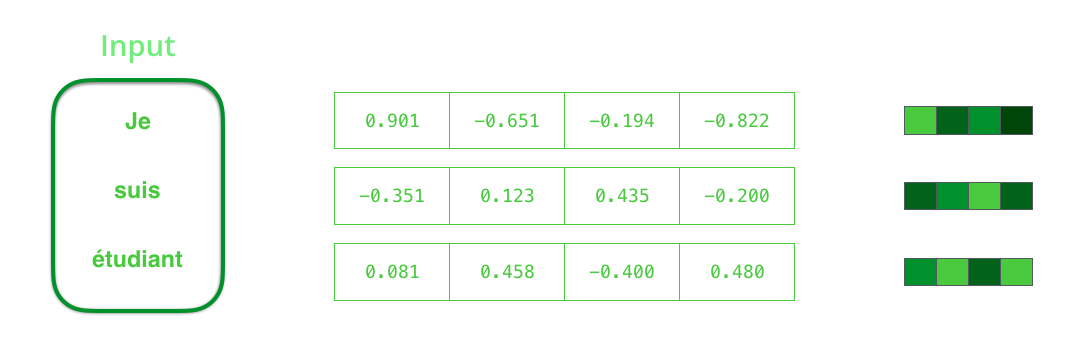
\includegraphics[width=0.8\textwidth]{example_word_embedding.png}
%\vspace{-10pt}
%\caption{\footnotesize Example Word Embeddings. From \emph{Visualizing Neural Machine Translation Mechanics of Seq2Seq Models with Attention}, by Jay Alammar, 2018. \url{http://jalammar.github.io/visualizing-neural-machine-translation-mechanics-of-seq2seq-models-with-attention/}. Copyright 2018 by Jay Alammar.}
%\vspace{-10pt}
%\label{fig:exampleWordEmb}
%\end{figure}

From Rudolph et al. (2016), ``each term in a vocabulary is associated with two latent vectors, an \emph{embedding} and a \emph{context vector}. These two types of vectors govern conditional probabilities that relate each word to its surrounding context." 
Rudolph and Blei (2017) explain that a word's conditional probability combines its \emph{embedding} and \emph{context vectors} of surrounding words, with different methods combining them differently. Subsequently, word embeddings are fitted to text by maximizing conditional probabilities of observed text. 

\subsection{Static Embeddings vs. Contextual Embeddings} \label{sec:StaticVsContextualEmb}

\subsubsection{What is Polysemy?} \label{sec:Polysemy}

\textbf{Polysemy} means a word can have distinct meanings. A related concept in NLP we will also use is the \textbf{distributional hypothesis}, which states meaning depends on context, and words occurring in same contexts have similar meaning (Wiedemann et al. 2019). 

\subsubsection{The Problem With Context-Free, Static Embeddings} \label{sec:ProblemWithStaticEmbs}

Classic word vectors, also called \textbf{static embeddings}, represent words in a low-dimensional continuous space by assigning a single vector per word, regardless of context (Ethayarajh, 2019). \nameref{sec:SkipGram} (Mikolov et al., 2013a) and \nameref{sec:Glove} (Pennington et al., 2014) produce these ``context-independent representations," as Peters et al. (2018) call them, since their word embedding matrix is trained to use co-occurring information in text, rather than the more dynamic \hyperref[sec:LanguageModels]{language modeling approach} (Batista, 2018). Although static embeddings still capture latent syntactic and semantic meaning by training over large corpora, they collapse all senses of a polysemous word into a single vector representation (Ethayarajh, 2019). For instance, the word ``plant" would have an embedding that is the ``average of its different contextual semantics relating to biology, placement, manufacturing, and power generation" (Neelakantan et al., 2015). 



\subsubsection{A Better Solution: Contextual Embeddings To Capture Polysemy} \label{sec:SolutionWithContextEmbs}

%In the Annual Review of Linguistics, Lenci (2018) states that ``distributional semantics is a usage-based model of meaning, based on the assumption that the statistical distribution of linguistic items in context plays a key role in characterizing their semantic behavior".

In different domains, context is defined differently. Rudolph et al. (2016) states that ``each data point $i$ has a \emph{context} $c$, which is a set of indices of other data points." In linguistics, the data point is taken to be a word and the context is the sequence of surrounding words. In neural data, the data point is neuron activity at a specific time and context is surrounding neuron activity. In shopping data, the data point refers to a purchase and context can mean other items in a basket (Rudolph et al., 2016). 

A \textbf{contextual word embedding (CWE)} is usually obtained using a \hyperref[sec:BidirectionalLM]{bidirectional language model (biLM)} to capture forward and backward history from surrounding phrases of a word (Antonio, 2019). While static embeddings are simple ``lookup tables", contextual embeddings contain word type information (Smith, 2019). CWEs avoid using a fixed word sense inventory, letting them: \textbf{($1$)} create a vector per word, and \textbf{($2$)} create a vector per word token in a context. Experimentally, CWEs capture word senses, letting Wiedemann et al. (2019) conclude CWEs are a more realistic model of natural language than static embeddings. Although contextualization models such as \nameref{sec:BERT}, \nameref{sec:XLNet}, and \textbf{ERNIE 2.0} differ widely, the field of NLP found that ``sentence or context-level semantics together with word-level semantics proved to be a powerful innovation" (Wiedemann et al., 2019). 

%Contextual embeddings have proven their superiority over static embeddings for many NLP tasks such as text classification (Zampieri et al., 2019) and sequence tagging (Akbig et al., 2018). 



